\documentclass[tikz,border=10pt]{standalone}
\usetikzlibrary{shapes.geometric, arrows.meta, positioning}

\tikzset{
  startstop/.style={rectangle, rounded corners, minimum width=3cm, minimum height=1cm,text centered, draw=black, fill=red!30},
  process/.style={rectangle, minimum width=3cm, minimum height=1cm, text centered, draw=black, fill=orange!30},
  decision/.style={diamond, minimum width=3cm, minimum height=1cm, text centered, draw=black, fill=green!30},
  arrow/.style={thick,->,>=stealth}
}

\begin{document}
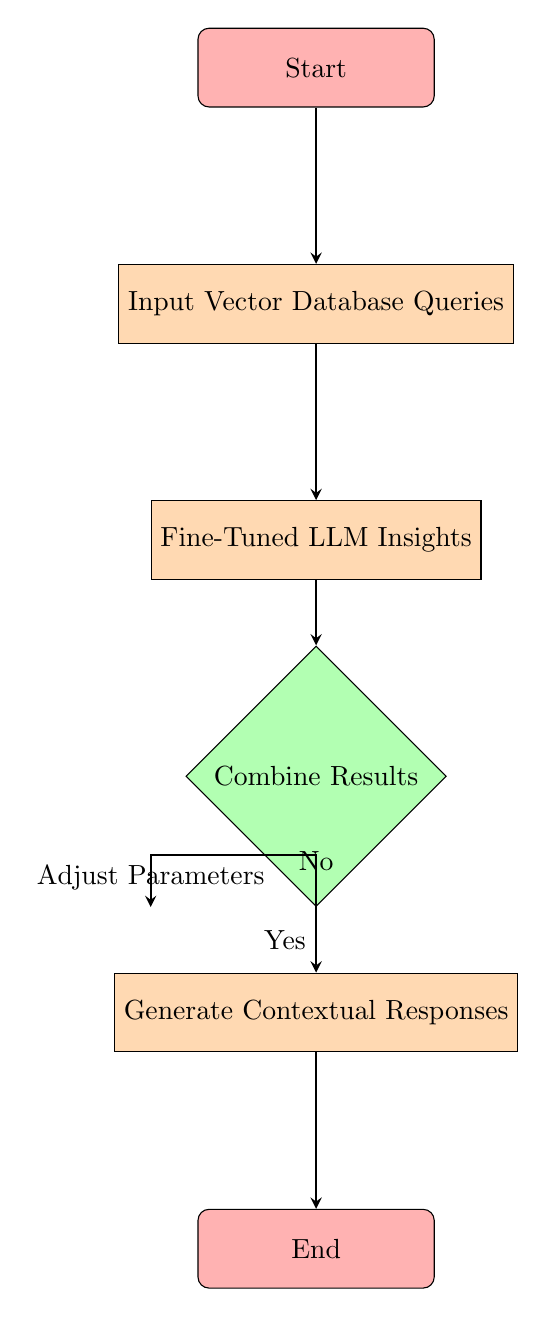
\begin{tikzpicture}[node distance=2cm]
    % Nodes
    \node (start) [startstop] {Start};
    \node (input) [process, below of=start, yshift=-1cm] {Input Vector Database Queries};
    \node (llm_insights) [process, below of=input, yshift=-1cm] {Fine-Tuned LLM Insights};
    \node (combine) [decision, below of=llm_insights, yshift=-1cm] {Combine Results};
    \node (output) [process, below of=combine, yshift=-1cm] {Generate Contextual Responses};
    \node (end) [startstop, below of=output, yshift=-1cm] {End};

    % Arrows
    \draw [arrow] (start) -- (input);
    \draw [arrow] (input) -- (llm_insights);
    \draw [arrow] (llm_insights) -- (combine);
    \draw [arrow] (combine) -- node[anchor=east] {Yes} (output);
    \draw [arrow] (combine) -- node[anchor=south] {No} ++(0,-1cm) -| node[anchor=north] {Adjust Parameters} (llm_insights.west |- combine.south);
    \draw [arrow] (output) -- (end);
\end{tikzpicture}
\end{document}